\documentclass[12pt,a4paper,openany]{article}
\usepackage[latin1]{inputenc}
\usepackage[T1]{fontenc}
\usepackage[spanish]{babel}
\usepackage{amsmath}
\usepackage{amsfonts}
\usepackage{amssymb}
\usepackage[backend=biber,style=ieee]{biblatex}
\addbibresource{Referencias.bib}
\usepackage{makeidx}
\usepackage{graphicx}
\usepackage{listings}
\usepackage[export]{adjustbox}
\usepackage{subcaption}
\usepackage{longtable}
\usepackage{array}
\lstloadlanguages{C, C++, csh, Java, vhdl}
\usepackage{color}
\definecolor{red}{rgb}{0.6,0,0} 
\definecolor{blue}{rgb}{0,0,0.6}
\definecolor{green}{rgb}{0,0.8,0}
\definecolor{cyan}{rgb}{0.0,0.6,0.6}
\definecolor{cloudwhite}{rgb}{1.0, 1.0,1.0}
\lstset{
language=vhdl,
basicstyle=\footnotesize\ttfamily,
numbers=left,
numberstyle=\tiny,
numbersep=5pt,
tabsize=2,
extendedchars=true,
breaklines=true,
frame=b,
stringstyle=\color{blue}\ttfamily,
showspaces=false,
showtabs=false,
xleftmargin=17pt,
framexleftmargin=17pt,
framexrightmargin=5pt,
framexbottommargin=4pt,
commentstyle=\color{green},
morecomment=[l]{--}, %use comment-line-style!
morecomment=[s]{/*}{*/}, %for multiline comments
showstringspaces=false,
morekeywords={ abstract, event, new, struct,
as, explicit, null, switch,
base, extern, object, this,
bool, false, operator, throw,
break, finally, out, true,
byte, fixed, override, try,
case, float, params, typeof,
catch, for, private, uint,
char, foreach, protected, ulong,
checked, goto, public, unchecked,
class, if, readonly, unsafe,
const, implicit, ref, ushort,
continue, in, return, using,
decimal, int, sbyte, virtual,
default, interface, sealed, volatile,
delegate, internal, short, void,
do, is, sizeof, while,
double, lock, stackalloc,
else, long, static,
enum, namespace, string},
keywordstyle=\color{cyan},
identifierstyle=\color{red},
backgroundcolor=\color{cloudwhite},
}
\usepackage{caption}
\DeclareCaptionFont{white}{\color{white}}
\DeclareCaptionFormat{listing}{\colorbox{blue}{\parbox{\textwidth}{\hspace{15pt}#1#2#3}}}
\captionsetup[lstlisting]{format=listing,labelfont=white,textfont=white, singlelinecheck=false, margin=0pt, font={bf,footnotesize}}
\usepackage[left=2.00cm, right=2.00cm, top=2.00cm, bottom=2.00cm]{geometry}
\author{Eduardo Hernandez Vergara}
\title{Tarea 1}
\begin{document}
		\begin{titlepage}
		\begin{figure}[!h]
			\begin{subfigure}{0.5\textwidth}
				
\includegraphics[width=0.2\linewidth, inner]{logoIPN}
			\end{subfigure}
			\begin{subfigure}{0.5\textwidth}
				
\includegraphics[width=0.2\linewidth, right]{logoESCOM}
			\end{subfigure}	
				
		\end{figure}		
		\centering
		\vspace{1cm}
		{\bfseries\LARGE INSTITUTO POLIT\'ECNICO NACIONAL \par}
		\vspace{1cm}
		{\scshape\Large Escuela Superior de Computo \par}
		\vspace{3cm}
		{\scshape\Huge Pr\'actica no. 1 ALU con Operaciones L\'ogicas, Aritm\'eticas y Corrimiento\par}
		\vspace{3cm}
		{\itshape\Large Arquitectura de Computadoras \par}
		\vfill
		{\Large Autores: \par}
		{\Large Hern\'andez Vergara, Eduardo \par}
		{\Large Rojas Cruz, Jos\'e \'Angel \par}
		{\Large Alcantara Covarrubias, Erik \par}
		{\Large Mart\'inez Alquicira, Mariana \par}
		\vfill
		{\Large Profesor: \par}
		{\Large Pastrana Fern\'andez Carlos Jes\'us \par}
		\vfill
		{\Large 15 de Octubre de 2022 \par}
	\end{titlepage}

	\tableofcontents
	 \section{Introduci\'on}
	\subsection{Objetivo}
		\setlength{\parindent}{1em}
		\setlength{\parskip}{10pt}
			El alumno realizar\'a una ALU,la que incluir\'a registros de corrimientos, l\'ogicos y aritm\'eticos la cual podr\'a realizar las operaciones con datos de 'n' bits especificados, tendr\'a una terminal que sirva para el control de carga.
	\subsection{Introducci\'on te\'orica}
		\subsubsection{Unidad Aritmetica L\'ogica (ALU)}
			La ALU es la parte de la computadora que realiza las operaciones l\'ogicas y aritmeticas de los datos. Todos los dem\'as elementos de los sistemas de computadoras (Control Unit, Registros, memoria, entrada/salida) son algunos de los datos que se le entregan a la ALU para que los procese y despu\'es los devuelva. Entonces, en un sentido, hemos alcanzado la esencia de una computadora cuando consideramos una ALU.
\vskip 1pt
	Una ALU y, en realidad todos los componentes electronicos en una computadora estan basados en el uso de simples dispositivos l\'ogicos digitales simples que pueden guardar digitos binarios y realizar simples operaciones l\'ogicas boleanas.
\vskip 1pt
	En la siguiente figura se muestra en t\'erminos generales, como esta interconectada la ALU con el resto del procesador. Los datos son presentados en los registros de la ALU, y los resultados de la operaci\'on se guarda en los registros. Estos registros son almacenados temporalmente mientras el procesador este conectado por rutas de se\~nal al ALU. Al ALU tambi\'en se le pueden configurar banderas como el resultado de una operaci\'on. Por ejemplo, la bandera de overflow se configura en 1 si el resultado excede el tama\~no del registro en donde va a ser almacenado. Los valores de estas banderas tambi\'en son almacenadas en los registros dentro del procesador. La unidad de control nos provee se\~nalesque controlan la operaci\'on del ALU y el movimiento de datos de entrada y salida del ALU.
	\begin{figure}[h]
			\centering		
			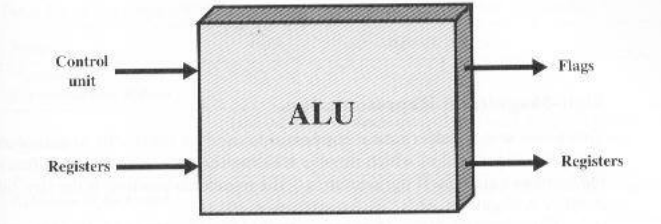
\includegraphics[width=\textwidth]{IOALU}
			\caption{Entradas y Salidas del ALU}
	\end{figure}
	\subsubsection{?`Qu\'e es VHDL?}
		VHDL es un lenguaje de dise\~no de software destinado a usarse en todas las fases del dise\~no de sistemas digitales. VHDL viene de VHSIC (Very High Speed Integrated Circuits) lenguaje descriptor de hardware. Su desarrollo empez\'o en 1983 con un contrato por parte del departamento de defenza de los Estados Unidos de \'America, y se volvi\'o un est\'andar de la IEEE en 1987.
	\subsubsection{?`Qu\'e es una FPGA?}
Una FPGA (Field Programmable Gate Array) es un complejo circuito integrado digital programable compuesto por bloques l\'ogicos configurables (CLB) y puertos de entrada/salida (IOB), cuya interconexi\'on y funcionalidad puede ser programada mediante un lenguaje de descripci\'on especializado.
\vskip 1pt
Su principal caracter\'istica y ventaja es que pueden reprogramarse para un trabajo espec\'ifico o cambiar sus requisitos despu\'es de haberse fabricado. Esto tambi\'en implica que en muchos casos se pueden hacer cambios f\'isicos sin hacer modificaciones costosas en la placa que lo soporta.
\vskip 1pt
B\'asicamente, una FPGA es un conjunto de m\'ultiples circuitos (l\'ogicos y de otros tipos) dispuestos matricialmente, cuyas interconexiones son programables por el usuario para la aplicaci\'on requerida. En una FPGA se programa su hardware, a diferencia de los microcontroladores / microprocesadores, en los que solo existe un hardware fijo y se programa su software (firmware).
\vskip 1pt
Hist\'oricamente, las FPGA fueron inventadas en el a\~no 1984 por Ross Freeman y Bernard Von Der Schmitt, cofundadores de la empresa Xilinx, fabricante de las mismas. Como resultado de numerosas evoluciones, la compa\~n\'ia produjo la primera familia de dispositivos l\'ogicos programables por el usuario, de prop\'osito general.
\vskip 1pt
Las FPGA, adem\'as de contener puertas l\'ogicas AND y OR, tienen memoria RAM, controladores de reloj, etc., por lo que son muy apropiadas para el dise\~no de sistemas embebidos con microprocesador. La compa\~n\'ia Xilinx ha evolucionado dicha tecnolog\'ia hasta convertirla en un nuevo concepto a tener en cuenta en ciertos entornos de trabajo.
	\subsection{Material y Equipo Empleado}
		\begin{itemize}
			\item 1 FPGA
			\item 1 Tarjeta de evaluaci\'on de pruebas \'o Protoboard microswitches con resistencias 10 KoHms, 20 leds con resistencias 330 oHms, 1 display de 4 digitos multiplexado de \'anodo com\'un.
			\item 1 eliminador de celular de 5v con cable mini usb.
			\item Quartus Prime Lite
		\end{itemize}
	
	\section{Desarrollo Experimental}
	\setlength{\parindent}{1em}
	\setlength{\parskip}{10pt}
	\subsection{Objetivo Espec\'ifico}
	\begin{enumerate}
		\item Desarrollar en la FPGA un programa en VHDL de una ALU,  en cu\'al se puedan seleccionar tres tipos de operaciones, L\'ogicas, Aritm\'eticas y Shifters, est\'as son:
		\begin{itemize}
			\item L\'ogicas (A y B de 10 bits):
			\begin{enumerate}
				\item Negaci\'on o Complemento a 1 de A.
				\item Complemento a 2 de A.
				\item AND entre A y B.
				\item OR entre A y B.
			\end{enumerate}
			\item Shifters (A de 10 bits):
			\begin{enumerate}
				\item LSL (Logical Shift Left).
				\item ASR. (Arithmetic Shift Right).
			\end{enumerate}
			\item Aritm\'eticas (A y B)
			\begin{enumerate}
				\item Suma 1 byte c/ carry out.
				\item Resta 1 byte.
				\item Multiplicaci\'on de 5 bits
			\end{enumerate}
		\end{itemize}
		\item Con los siguientes especificaciones:
		\begin{itemize}
			\item Realizar el programa en VHDL que incluya todas las operaciones b\'asicas (L\'ogicas, Shifters, Aritm\'eticas ) del tama\~no de dato correcto como se solicita en la descripci\'on.
			\item Recuerde que todas las operaciones anteriores deben funcionar como una unidad, para este inciso se deben programar todas las opciones por componentes o multi procesos.
			\item Para las opciones de corrimientos de debe incluir un clock para sincronizar los desplazamientos.
			\item Todas las entradas deben ser consideradas dependiendo de la operaci\'on a realizar, estas deber\'an ser introducidas por medio de microswitches.
			\item La asignaci\'on de pines se debe de hacer de acuerdo a la disponibilidad en las terminales de salida en la FPGA.
			\item La salida del bloque aritm\'etico se tendr\'a que ser desplegada en el display de 7 seg. 4 digitos y a su vez la salida de los shifters y la unidad l\'ogica se  mostrara \'unicamente mediante Leds.
		\end{itemize}
		\item Se manejara el mismo programa del inciso anterior pero ahora todas las operaciones tanto Aritm\'eticas,  shifters  o  l\'ogicas se  mostraran mediante mensaje  de  texto  pregrabado  en memoria ROM indexada en VHDL para el texto identificador de la operaci\'on por ejemplo: SunnA,  rEstA,  nnulti,  And, or,  not,  Co1,  Co2,  ror,  roL,  LSL,LSren  tipo  ventana  deslizante display de 4 d\'igitos de tipo \'anodo com\'un de 7 seg. El cual se multiplexar\'a para que se despliegue 5 segundos antes de mostrar el resultado de la operaci\'on. Cada  una  de  las  letras  ser\'a  almacenada  en  un  solo  byte,  y  se  multiplexar\'a similar  a  los n\'umeros pero con ventana deslizante que significa que el mensaje se desplaza para mostrar todas las letras durante 5 segundos de forma autom\'atica antes de mostrar el resultado.
	\end{enumerate}
\clearpage
	\section{C\'odigo}
	\begin{lstlisting}[language={vhdl}, caption={Barrel Shifter (Prototipo)}, label={Script}]
LIBRARY IEEE;
USE IEEE.std_logic_1164.ALL;
USE IEEE.numeric_std.ALL;

ENTITY barrelShifters IS
    PORT (
        a : IN STD_LOGIC_VECTOR(9 DOWNTO 0);
        cntrl, clk, iniciar : IN STD_LOGIC;
        salidaLC : OUT STD_LOGIC;
        salShifters : OUT STD_LOGIC_VECTOR(9 DOWNTO 0)
    );
END ENTITY barrelShifters;

ARCHITECTURE shifters OF barrelShifters IS

    SIGNAL contador : INTEGER RANGE 0 TO 49999999 := 0;
    SIGNAL aux : STD_LOGIC_VECTOR(9 DOWNTO 0) := "0000000000";
    SIGNAL salidMed : STD_LOGIC;

BEGIN
    --Mi divisor de frecuencias
    DivisorFrecuencia : PROCESS (clk, iniciar)
    BEGIN
        IF iniciar = '0' THEN
            salidMed <= '0';
            contador <= 0;
        ELSIF rising_edge(clk) THEN
            IF contador = 49999999 THEN
                contador <= 0;
                salidMed <= NOT salidMed;
            ELSE
                contador <= contador + 1;
            END IF;
        END IF;
    END PROCESS DivisorFrecuencia;

    salidaLC <= salidaMed;
    --Las opciones del shifter
    Shifter : PROCESS (salidaMed, iniciar, a, cntrl)
    BEGIN
        IF iniciar = '0' THEN
            aux <= "0000000000";
        ELSIF rising_edge(salidaMed) THEN
            IF (cntrl = '0') THEN
                aux <= a(8 DOWNTO 0) & '0'; --LSL
            ELSE
                aux <= a(9) & a(9 DOWNTO 1);-- Arithmetic Shifter Right
            END IF;
        END IF;
    END PROCESS Shifter;

    salShifters <= aux;
    a <= aux;
END ARCHITECTURE shifters;
	\end{lstlisting}
\begin{lstlisting}[language={vhdl}, caption={Display Operaciones (Prototipo)}, label={Script}]
-- PROTOTIPO
LIBRARY IEEE;
USE IEEE.std_logic_1164.ALL;
USE IEEE.numeric_std.ALL;
ENTITY displayOperaciones IS
    PORT (
        cntrlSeg : IN STD_LOGIC_VECTOR(0 TO 1);
        cntrlArt : IN STD_LOGIC_VECTOR(0 TO 1);
        cntrlShf : IN STD_LOGIC;
        cntrlLog : IN STD_LOGIC_VECTOR(0 TO 1);
        d0, d1, d2, d3 : OUT STD_LOGIC_VECTOR(0 TO 6)
    );
END ENTITY displayOperaciones;
ARCHITECTURE dOperaciones OF displayOperaciones IS
    SIGNAL ad0, ad1, ad2, ad3 : STD_LOGIC_VECTOR(0 TO 6);
BEGIN
    ProcDisplay : PROCESS (cntrlSeg, cntrlArt, cntrlShf, cntrlLog, ad1, ad2, ad0, ad3)
    BEGIN
        IF cntrlSeg = "00" THEN --Artimethic
            IF cntrlArt = "00" THEN --Suma
                ad0 <= "0100100"; --S Anodo
                ad1 <= "1000001"; --U Anodo
                ad2 <= "1101010"; --n Andodo
                ad3 <= "1101010"; --n Andodo
            ELSIF cntrlArt = "01" THEN -- Resta
                ad0 <= "1111010"; --r Anodo
                ad1 <= "0110000"; --E Anodo
                ad2 <= "0100100"; --S Anodo
                ad3 <= "1110000"; --t Andodo
            ELSIF cntrlArt = "10" THEN --Mult
                ad0 <= "1101010"; --n Anodo
                ad1 <= "1101010"; --n Anodo
                ad2 <= "1000001"; --U Anodo
                ad3 <= "1110001"; --L Andodo
            END IF;
        ELSIF cntrlSeg = "01" THEN --Shifter
            IF cntrlShf = '0' THEN -- LSL
                ad0 <= "1110001"; --L Anodo
                ad1 <= "0100100"; --S Anodo
                ad2 <= "1110001"; --L Andodo
                ad3 <= "1111111"; --NULL Andodo
            ELSE --ASR
                ad0 <= "0001000"; --A Anodo
                ad1 <= "0100100"; --S Anodo
                ad2 <= "1111010"; --r Andodo
                ad3 <= "1111111"; --NULL Andodo
            END IF;
        ELSIF cntrlSeg = "10" THEN --Logic
            IF cntrlLog = "00" THEN --NOT
                ad0 <= "1101010"; --n Anodo
                ad1 <= "1100010"; --o Anodo
                ad2 <= "1110000"; --t Andodo
                ad3 <= "1111111"; --null Andodo
            ELSIF cntrlLog = "01" THEN -- COMP2
                ad0 <= "0110001"; --C Anodo
                ad1 <= "1100010"; --o Anodo
                ad2 <= "0011000"; --P Anodo
                ad3 <= "0010010"; --2 Andodo
            ELSIF cntrlLog = "10" THEN --AND
                ad0 <= "0001000"; --A Anodo
                ad1 <= "1101010"; --n Anodo
                ad2 <= "1000010"; --d Anodo
                ad3 <= "1111111"; --null Andodo
            ELSIF cntrlLog = "11" THEN --OR
                ad0 <= "1111111"; --null Anodo
                ad1 <= "1100010"; --o Anodo
                ad2 <= "1111010"; --r Anodo
                ad3 <= "1111111"; --null Andodo
            END IF;
        END IF;
    END PROCESS ProcDisplay;
    d0 <= ad0;
    d1 <= ad1;
    d2 <= ad2;
    d3 <= ad3;
END ARCHITECTURE dOperaciones;
	\end{lstlisting}
	\section{Conclusiones}
	\subsection{Conclusiones Generales}
	Eget lorem dolor sed viverra ipsum nunc. Ipsum dolor sit amet consectetur. Ipsum dolor sit amet consectetur adipiscing elit. Est ultricies integer quis auctor elit sed vulputate mi sit. Sit amet venenatis urna cursus eget. Morbi quis commodo odio aenean sed adipiscing. In dictum non consectetur a erat. Eu lobortis elementum nibh tellus molestie nunc non blandit massa. Neque ornare aenean euismod elementum nisi quis eleifend. Nisl suscipit adipiscing bibendum est ultricies integer quis. Sodales neque sodales ut etiam sit amet nisl purus in.
	\subsection{Conclusiones Eduardo Hern\'andez Vergara}
		Lorem ipsum dolor sit amet, consectetur adipiscing elit, sed do eiusmod tempor incididunt ut labore et dolore magna aliqua. Consectetur purus ut faucibus pulvinar elementum integer. Ullamcorper velit sed ullamcorper morbi tincidunt ornare. In fermentum et sollicitudin ac. Magna ac placerat vestibulum lectus mauris. Semper quis lectus nulla at volutpat diam ut. Gravida arcu ac tortor dignissim convallis aenean et tortor at. Integer eget aliquet nibh praesent tristique magna. Sed velit dignissim sodales ut eu sem integer vitae justo. Vel fringilla est ullamcorper eget nulla facilisi etiam dignissim diam.
	\subsection{Conclusiones Jos\'e \'Angel Rojas Cruz}
	Ultricies mi quis hendrerit dolor magna eget est lorem ipsum. Velit egestas dui id ornare arcu odio. Neque sodales ut etiam sit amet nisl purus in mollis. Nec ultrices dui sapien eget mi proin sed libero enim. Sit amet risus nullam eget felis eget nunc lobortis. Velit dignissim sodales ut eu sem. Lorem donec massa sapien faucibus et molestie. Quis varius quam quisque id diam vel quam elementum pulvinar. Netus et malesuada fames ac turpis. Posuere sollicitudin aliquam ultrices sagittis orci a. Scelerisque felis imperdiet proin fermentum leo vel orci porta. Et malesuada fames ac turpis egestas maecenas.
	\subsection{Conclusiones Erik Alcantara Covarrubias (revisar)}
	Elementum integer enim neque volutpat. Congue nisi vitae suscipit tellus mauris a diam maecenas. Neque egestas congue quisque egestas diam in arcu cursus euismod. Mauris commodo quis imperdiet massa tincidunt nunc pulvinar sapien. Tempus egestas sed sed risus pretium quam vulputate dignissim suspendisse. Tincidunt vitae semper quis lectus nulla at. Vitae et leo duis ut diam. Sagittis id consectetur purus ut faucibus pulvinar elementum integer. Tortor consequat id porta nibh venenatis cras sed felis eget. Sit amet consectetur adipiscing elit pellentesque habitant morbi tristique. Sagittis aliquam malesuada bibendum arcu vitae elementum curabitur vitae nunc. Dui ut ornare lectus sit amet est placerat in. Dignissim sodales ut eu sem. Tincidunt eget nullam non nisi est sit amet facilisis magna. Tortor vitae purus faucibus ornare suspendisse sed nisi.
	\subsection{Conclusiones Mariana Alquisira (revisar)}
	Congue nisi vitae suscipit tellus mauris a. Hendrerit dolor magna eget est lorem ipsum dolor sit amet. Tortor at risus viverra adipiscing at. Diam maecenas ultricies mi eget mauris pharetra. Sed enim ut sem viverra aliquet eget sit amet tellus. Egestas fringilla phasellus faucibus scelerisque eleifend. Laoreet suspendisse interdum consectetur libero. Nec feugiat in fermentum posuere urna nec tincidunt praesent. Quis commodo odio aenean sed adipiscing. Consectetur adipiscing elit ut aliquam. Odio morbi quis commodo odio aenean. Morbi tincidunt augue interdum velit euismod in pellentesque massa. Sit amet purus gravida quis. Tempor commodo ullamcorper a lacus.
	\section{Referencias}
\begin{thebibliography}{0}
	\bibitem{Stallings2003}
	Stallings, W. (2003). \textit{Computer Organization and Architecture}. Pearson Education International.
	\bibitem{Jasinski2015}
	Jasinski, R. (2015). \textit{Efective Coding with VHDL: principles and best practice}. The MIT Press.
\bibitem{AkkaND}
	Akka Technologies. (n.d.). \textit{FPGA: qu\'e es y cu\'ales son las caracter\'isticas de este componente. [online]}. Available at: https://www.akka-technologies.com/fpga/ [Accessed 16 Oct. 2022]..
\end{thebibliography}
\printbibliography
\end{document}